\section{Experiment}
\label{sec:experiment}

\begin{figure}[h]
	\centering
	\label{fig:dataset}
	\begin{tikzpicture}
		[every axis/.style={
			ybar,
			scale only axis,
			ymin=0, ymax= 130000,
			width=0.5\textwidth,
			height=0.4\textwidth,
			legend style={at={(20em,5em)}, anchor=east},
			bar width=1em,
			scaled y ticks=false,
			xtick=data,
			font=\scriptsize,
			symbolic x coords={FB15k,FB15k-237,WN18,WN18RR,YAGO3-10},
			nodes near coords,
			nodes near coords align={vertical},
		}]
		\pgfplotsset{
			compat=newest,
			major grid style=blue,
			xlabel near ticks,
			ylabel near ticks
		}
		
		\begin{axis}[]
			\addplot [fill=awesome] coordinates {
				(FB15k,14951)
				(FB15k-237,14541)
				(WN18,40943)
				(WN18RR,40559)
				(YAGO3-10,123182)
			};
			\addplot [fill=azure] coordinates {
				(FB15k,1345)
				(FB15k-237,237)
				(WN18,18)
				(WN18RR,11)
				(YAGO3-10,37)
			};
			\legend{Entities, Relations}
		\end{axis}
	\end{tikzpicture}
	
\end{figure}


In this section, we describe the datasets used for our empirical evaluation, along with a comparison against notable existing methods as reported in \autoref{tab:graphEmbeddingTechCompare}. Additionally, we evaluate our two proposed approaches for injecting new knowledge into the knowledge graph. Specifically, we treat the test set as a batch of new knowledge to be added, and use the validation set to re-evaluate the effectiveness of our method. Detailed results are presented in \autoref{tab:resultOnFreeBase} and \autoref{tab:resultOnWordNet}.


\begin{table}[H]
	\begin{center}
		%		\resizebox{\linewidth}{!}{%
			\begin{tabular}{llllll}
				\hline
				&          &           & \multicolumn{3}{l}{\# Edges}    \\ \cline{4-6}
				
				Dataset   & Entities & Relations & Training & Validation & Test    \\ \hline
				FB15k     & 14,951   & 1,345     & 483,142  & 50,000     & 59,071 \\
				FB15k-237 & 14,541   & 237       & 272,115  & 17,535     & 20,466  \\
				WN18      & 40,943   & 18        & 141,442  & 5,000      & 5,000   \\
				WN18RR    & 40,559   & 11        & 86,835   & 3,034       & 3,134    \\
				YAGO3-10    & 123,182   & 37        & 1,079,040   & 5,000       & 5,000  \\
				\hline
			\end{tabular}
			%		}
		\caption{Dataset Information}
		\label{tab:datasetInfo}
	\end{center}
\end{table}

%\section{Các tập dữ liệu huấn luyện}
\section{Training Datasets}
\label{sec:DataTraining}

\begin{figure}[H]
	\centering
	\label{fig:dataset_split}
	
	\pgfplotstableread[row sep=\\,col sep=&]{
		Dataset & Entities & Relations & Training & Validation & Test\\
		FB15k & 14951 & 1345 & 483142 & 50000 & 59071  \\
		FB15k-237 & 14541 & 237 & 272115 & 17535 & 20466  \\
		WN18 & 40943 & 18 & 141442 & 5000 & 5000  \\
		WN18RR & 40559 & 11 & 86835 & 3034 & 3134  \\
		YAGO3-10 & 123182 & 37 & 1079040 & 5000 & 5000  \\
	}\mydata
	\resizebox{\linewidth}{!}{%
		\begin{tikzpicture}
			\begin{axis}[
				xbar stacked,
				tick align = outside, xtick pos = left,
				scale only axis,
				scaled x ticks=false,
				every node near coord/.style={/pgf/number format/fixed},
				xticklabel style={/pgf/number format/fixed},
				width=\textwidth,
				height=0.3\textwidth,
				font=\scriptsize,
				legend style={at={(0.5,-0.15)}, anchor=north, legend columns=-1},
				bar width=1.5em,
				ytick=data,
				y dir = reverse,
				yticklabels from table={\mydata}{Dataset},
				]
				\addplot[fill=azure] table [y expr=\coordindex,x=Training]{\mydata};
				\addplot+[fill=awesome] table [y expr=\coordindex,x=Validation]{\mydata};
				\addplot+[fill=amber,
				point meta=x,
				nodes near coords = {\pgfmathprintnumber[precision=1]{\pgfplotspointmeta}},
				nodes near coords align={anchor=west},
				every node near coord/.append style={
					black,
					fill=white,
					fill opacity=0.75,
					text opacity=1,
					outer sep=\pgflinewidth
				}] table [y expr=\coordindex,x=Test]{\mydata};
				\legend{Training, Validation, Test};
			\end{axis}
		\end{tikzpicture}
	}
\end{figure}


In our experiments, we evaluate our approach on four widely used benchmark datasets: FB15k, FB15k-237 (\cite{toutanova2015observed}), WN18, and WN18RR (\cite{dettmers2018convolutional}). Each dataset is divided into three subsets: training, validation, and test sets. Detailed statistics for these datasets are presented in \autoref{tab:datasetInfo}. 

Each dataset consists of a collection of triples in the form \(\langle head, relation, tail \rangle\). FB15k and WN18 are derived from the larger knowledge bases FreeBase and WordNet, respectively. However, they contain a large number of inverse relations, which allow most triples to be easily inferred. To address this issue and to better reflect real-world link prediction scenarios, FB15k-237 and WN18RR were constructed by removing such inverse relations.

\subsection{FB15k Dataset}

This dataset was constructed by the research group of A. Bordes and N. Usunier \cite{bordes2013translating} by extracting data from the Wikilinks database\footnote{https://code.google.com/archive/p/wiki-links/}. The Wikilinks database contains hyperlinks to Wikipedia articles, comprising over 40 million mentions of approximately 3 million entities. The authors extracted all facts related to a given entity that is mentioned at least 100 times across different documents, along with all facts associated with those entities (including child entities mentioned in the corresponding Wikipedia articles), excluding attributes such as dates, proper nouns, etc. 

Entities with degree \(n\) were normalized by converting multi-way edges into sets of binary relations—enumerating all edges and relations between each pair of nodes.

%\ The dataset is randomly split into three subsets: the training set includes 1345 relations, 14,834 head entities, and 14,903 tail entities; the test set includes 916 relations, 11,886 head entities, and 11,285 tail entities; and the validation set includes 961 relations, 12,297 head entities, and 11,825 tail entities.

\subsection{FB15k-237 Dataset}

This dataset is a subset of FB15k, constructed by Toutanova and Chen \cite{toutanova2015observed}, motivated by the observation that FB15k suffers from test leakage, where models are exposed to test facts during training. This issue arises due to the presence of duplicate or inverse relations in FB15k. FB15k-237 was created to provide a more challenging benchmark. The authors selected facts related to the 401 most frequent relations and eliminated all redundant or inverse relations. Additionally, they ensured that no entities connected in the training set were directly linked in the test and validation sets.

%\ The training set includes 237 relations, 13,781 head entities, and 13,379 tail entities; the test set includes 223 relations, 7,652 head entities, and 5,804 tail entities; and the validation set includes 224 relations, 8,171 head entities, and 6,376 tail entities.



\subsection{WN18 Dataset}

\begin{center}
	\resizebox{\linewidth}{!}{%
		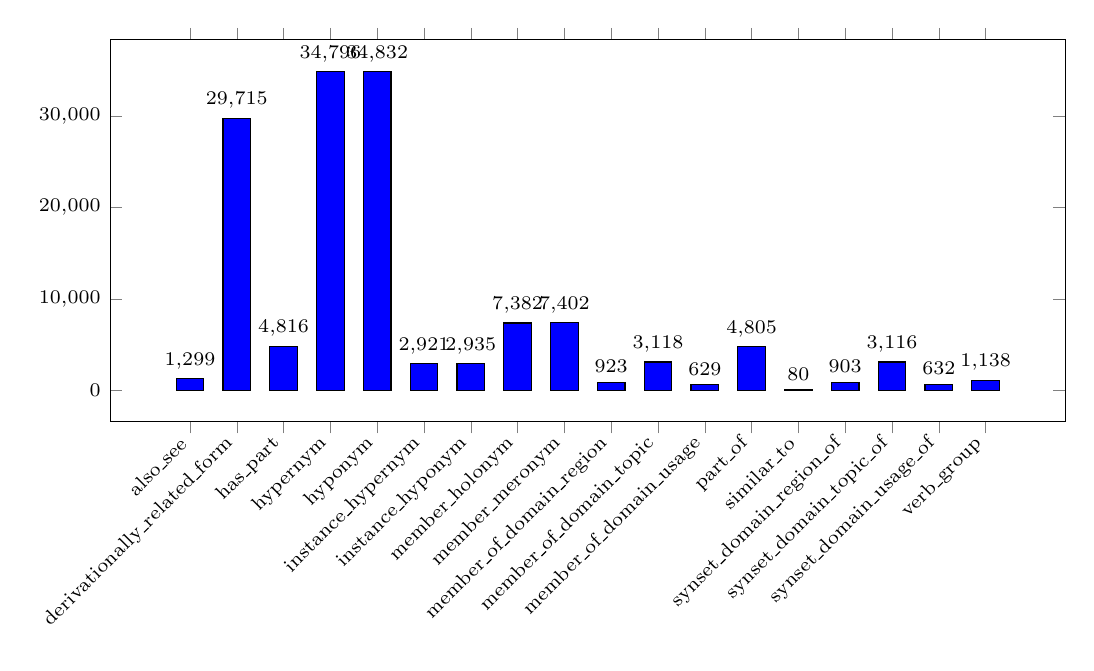
\begin{tikzpicture}
			[every axis/.style={
				ybar,
				scale only axis,
				width=\textwidth,
				height=0.4\textwidth,
				xtick=data,
				x tick label style={rotate=45, anchor=east},
				legend style={at={(20em,5em)}, anchor=east},
				bar width=1em,
				scaled y ticks=false,
				font=\scriptsize,
				symbolic x coords={
					also\_see,
					derivationally\_related\_form,
					has\_part,
					hypernym,
					hyponym,
					instance\_hypernym,
					instance\_hyponym,
					member\_holonym,
					member\_meronym,
					member\_of\_domain\_region,
					member\_of\_domain\_topic,
					member\_of\_domain\_usage,
					part\_of,
					similar\_to,
					synset\_domain\_region\_of,
					synset\_domain\_topic\_of,
					synset\_domain\_usage\_of,
					verb\_group},
				nodes near coords,
				nodes near coords align={vertical},
			}]
			\pgfplotsset{
				compat=newest,
				major grid style=blue,
				xlabel near ticks,
				ylabel near ticks
			}
			
			\begin{axis}[]
				\addplot [fill=blue] coordinates {
					(also\_see,1299)
					(derivationally\_related\_form,29715)
					(has\_part,4816)
					(hypernym,34796)
					(hyponym,34832)
					(instance\_hypernym,2921)
					(instance\_hyponym,2935)
					(member\_holonym,7382)
					(member\_meronym,7402)
					(member\_of\_domain\_region,923)
					(member\_of\_domain\_topic,3118)
					(member\_of\_domain\_usage,629)
					(part\_of,4805)
					(similar\_to,80)
					(synset\_domain\_region\_of,903)
					(synset\_domain\_topic\_of,3116)
					(synset\_domain\_usage\_of,632)
					(verb\_group,1138)
				};
			\end{axis}
		\end{tikzpicture}
	}
\end{center}

This dataset was introduced by the authors of TransE \cite{bordes2013translating}, and is extracted from WordNet\footnote{https://wordnet.princeton.edu/}, a lexical knowledge graph ontology designed to provide a dictionary/thesaurus to support NLP tasks and automated text analysis. In WordNet, entities correspond to synsets (i.e., \textit{word senses}), and relations represent lexical connections among them (e.g., “hypernym”). 

To construct WN18, the authors used WordNet as a starting point and iteratively filtered out entities and relations that were infrequently mentioned.


%Tập dữ liệu được chia ngẫu nhiên thành 3 tập: tập training với 18 relations, 40504 head entities, và 40551 tail entities, tập test gồm 18 relations, 4262 head entities, and 4338 tail entities, tập vadiation gồm 18 relations, 4349 head entities, and 4263 tail entities.

\subsection{WN18RR Dataset}

This dataset is a subset of WN18, constructed by DeŠmers et al.\cite{dettmers2017convolutional}, who also addressed the issue of test leakage in WN18. To tackle this issue, they created the WN18RR dataset, which is significantly more challenging, by applying a similar methodology to that used in FB15k-237 \cite{toutanova2015observed}.

\section{Evaluation Metrics}

In this section, we describe the evaluation metrics, experimental environment, and datasets used to assess the proposed method. These metrics are widely adopted for evaluating link prediction models on knowledge graphs. We compare our approach against four other state-of-the-art methods reported in \cite{rossi2020knowledge}.

\subsubsection{Hits@K (H@K)}

This metric measures the proportion of correct predictions whose rank is less than or equal to the threshold \(K\):
\[
H@K = \frac{\mid \{ q \in Q : \text{rank}(q) \leq K \} \mid}{\mid Q \mid}
\]

\subsubsection{Mean Rank (MR)}

This metric calculates the average rank of the correct entity in the prediction. A lower value indicates better model performance:
\[
MR = \frac{1}{\mid Q \mid} \sum_{q \in Q} \text{rank}(q)
\]
Here, \(\mid Q \mid\) denotes the total number of queries, which equals the size of the test or validation set. During evaluation, we perform both head and tail entity predictions for each triple. For example, we predict both \(\langle ?,~ \text{relation},~ \text{tail} \rangle\) and \(\langle \text{head},~ \text{relation},~ ? \rangle\). The variable \(q\) denotes a query, and \(\text{rank}(q)\) indicates the rank position of the correct entity. The final MR score is the average rank over all head and tail predictions.

Clearly, this metric ranges from \([1,~|\text{number of entities}|]\), as a node can connect to at most \(n-1\) other nodes plus a self-loop. However, this metric is highly sensitive to outliers, as certain relations may yield extremely low rankings for correct entities. To address this issue, our method—as well as other recent works—also adopts the Mean Reciprocal Rank (MRR) metric.


\subsubsection{Mean Reciprocal Rank (MMR)}
This is the Mean Reciprocal Rank (MRR), calculated as the reciprocal of the average rank obtained for a correct prediction. Higher values indicate better model performance. Since this metric takes the reciprocal of each rank, it helps mitigate the noise sensitivity encountered in the Mean Rank (MR) metric:
\[
MRR =\frac{1}{\mid Q \mid} \sum_{q \in Q} \frac{1}{\text{rank}(q)}
\]

\section{Training Methodology}

%\subsection{Training with the AnyBURL Model}

\subsection{Training with the KBGAT Model}

We first initialize the entity and relation embeddings using the TransE model \cite{bordes2013translating}. To construct negative (invalid) triples, we randomly replace either the head or tail entity in a valid triple with another entity sampled from the entity set.

The training process is divided into two phases. The first phase serves as an encoder, transforming the initialized embeddings into new embeddings that aggregate neighborhood information using the KBGAT model. This produces updated embeddings for both entities and relations. The second phase serves as a decoder, performing link prediction by incorporating $n$-hop neighborhood information. This enables the model to better aggregate context from neighboring entities. Furthermore, we incorporate auxiliary relations to enrich the local structure in sparse graphs.

We use the Adam optimizer with a learning rate of $\mu = 0.001$. The final embedding dimension for both entities and relations is set to 200. The optimal hyperparameters are determined via grid search, as detailed in \autoref{appendix:Appendix1}.


\section{Experimental Results}
\label{sec:Experiment}

As previously mentioned, our rule-based model can be fully executed on a standard laptop. In our experiment, the machine configuration was as follows: T480, Core i5 8th Gen, 16GB RAM, 4 cores and 8 threads. The source code was implemented in Python version 3.6, utilizing only built-in Python functions without any third-party libraries. The experiments were conducted on four widely-used datasets: FB15k, FB15-237, WN18, and WN18RR. Detailed information about these datasets is provided in \autoref{sec:DataTraining} under the training datasets section.

As described in \autoref{alg:GenerateRules}, the AnyBURL algorithm learns rules generated within a user-configurable time interval. Here, we set the training time to 1000 seconds (approximately 17 minutes), with saturation (SAT) set to \(0.85\), confidence threshold Q set to \(0.05\), and sample size S configured as (\(\frac{1}{10}~ \text{of the training set}\)). With this setup, our Python version of the model produced results comparable to the Java version developed by Meilicke, Christian et al. \cite{burl}, which was configured similarly but trained for only 100 seconds. The difference in training time is primarily due to performance differences between Python and Java. We chose Python because it is the primary language used in many recent artificial intelligence models and provides convenience for performance comparison and evaluation with other deep learning methods, most of which are also implemented in Python.



\begin{table}[H]
	\begin{center}
		\caption{Experimental results on the FB15k and FB15k-237 datasets}
		\label{tab:resultOnFreeBase}%
		\resizebox{\linewidth}{!}{%
			\begin{tabular}{l|l|l|l|l|l|l|l|l|}
				\cline{2-9}
				& \multicolumn{4}{c|}{\textbf{FB15k}}                   & \multicolumn{4}{c|}{\textbf{FB15k-237}}                   \\ \cline{2-9} 
				& \textbf{H@1} & \textbf{H@10} & \textbf{MR} & \textbf{MRR} & \textbf{H@1} & \textbf{H@10} & \textbf{MR} & \textbf{MRR} \\ \hline
				\multicolumn{1}{|l|}{ComplEx} & 81.56        & 90.53         & 34          & 0.848        & 25.72        & 52.97         & 202        & 0.349        \\ \hline
				\multicolumn{1}{|l|}{TuckER}  & 72.89        & 88.88         & 39          & 0.788        & 25.90        & 53.61         & 162         & 0.352        \\ \hline
				\multicolumn{1}{|l|}{TransE}  & 49.36        & 84.73         & 45          & 0.628        & 21.72        & 49.65         & 209         & 0.31        \\ \hline
				\multicolumn{1}{|l|}{RoteE}   & 73.93        & 88.10         & 42          & 0.791        & 23.83        & 53.06         & 178         & 0.336        \\ \hline
				\multicolumn{1}{|l|}{ConvKB}  & 59.46        & 84.94         & 51         & 0.688        & 21.90        & 47.62         & 281         &0.305        \\ \hline
				\multicolumn{1}{|l|}{\textbf{KBGAT}}     &  70.08            &     91.64    &  38    &   0.784    & 36.06     &    58.32   &  211  &    0.4353  \\ \hline
				\multicolumn{1}{|l|}{\textbf{AnyBURL}}    & 79.13        & 82.30         & 285         & \underline{0.824}        & 20.85        & 42.40         & 490         & 0.311        \\ \hline
			\end{tabular}
		}
	\end{center}
\end{table}


\begin{table}[H]
	\begin{center}
		\caption{Experimental results on the WN18 and WN18RR datasets}
		\label{tab:resultOnWordNet}%
		\resizebox{\linewidth}{!}{%
			\begin{tabular}{l|l|l|l|l|l|l|l|l|}
				\cline{2-9}
				& \multicolumn{4}{c|}{\textbf{WN18}}                              & \multicolumn{4}{c|}{\textbf{WN18RR}}                            \\ \cline{2-9} 
				& \textbf{H@1}   & \textbf{H@10}  & \textbf{MR}  & \textbf{MRR}   & \textbf{H@1}   & \textbf{H@10}  & \textbf{MR}  & \textbf{MRR}   \\ \hline
				\multicolumn{1}{|l|}{ComplEx} & 94.53          & 95.50          & 3623         & 0.349          & 42.55          & 52.12          & 4909         & 0.458          \\ \hline
				\multicolumn{1}{|l|}{TuckER}  & 94.64          & 95.80          & 510          & 0.951          & 42.95          & 51.40          & 6239         & 0.459          \\ \hline
				\multicolumn{1}{|l|}{TransE}  & 40.56          & 94.87          & 279          & 0.646          & 2.79           & 94.87          & 279          & 0.646          \\ \hline
				\multicolumn{1}{|l|}{RoteE}   & 94.30          & 96.02          & 274          & 0.949          & 42.60          & 57.35          & 3318         & 0.475          \\ \hline
				\multicolumn{1}{|l|}{ConvKB}  & 93.89          & 95.68          & 413          & 0.945          & 38.99          & 50.75          & 4944         & 0.427          \\ \hline
				\multicolumn{1}{|l|}{\textbf{KBGAT}}     &                &        &        &                &       35.12         &        57.01         &      \underline{1974}       &  0.4301           \\ \hline
				\multicolumn{1}{|l|}{\textbf{AnyBURL}}    &  93.96 & 95.07 & \textbf{230} & \textbf{0.955} & \textbf{44.22} & 54.40 & 2533 & \underline{0.497} \\ \hline
			\end{tabular}
		}
	\end{center}
\end{table}


\autoref{tab:resultOnFreeBase} and \autoref{tab:resultOnWordNet} describe our experimental results with the \(H@K\) metrics along with the experimental results of other methods mentioned in the survey \cite{rossi2020knowledge}.


\begin{table}[H]
	\begin{center}
		\caption{Accuracy results of the two new knowledge addition strategies}
		\label{tab:CompareAccuracy}%
		\resizebox{0.8\columnwidth}{!}{%
			\begin{tabular}{ll|l|l|l|}
				\cline{3-5}
				&        & \textbf{AnyBURL} & \textbf{Batch edge AnyBURL} & \textbf{Edge AnyBURL} \\ \hline
				\multicolumn{1}{|l|}{\multirow{3}{*}{\textbf{FB-15k}}}    & hit@10 & 82.22                  & 82.48               & 83.08               \\ \cline{2-5} 
				\multicolumn{1}{|l|}{}                                    & MR     & 285                    & 250                 & 220                 \\ \cline{2-5} 
				\multicolumn{1}{|l|}{}                                    & MRR    & 0.824                  & 0.853               & 0.866               \\ \hline
				\multicolumn{1}{|l|}{\multirow{3}{*}{\textbf{FB15k-237}}} & hit@10 & 42.40                  & 43.40               & 43.51               \\ \cline{2-5} 
				\multicolumn{1}{|l|}{}                                    & MR     & 490                    & 472                 & 441                 \\ \cline{2-5} 
				\multicolumn{1}{|l|}{}                                    & MRR    & 0.311                  & 0.353               & 0.377               \\ \hline
				\multicolumn{1}{|l|}{\multirow{3}{*}{\textbf{WN18}}}      & hit@10 & 95.07                  & 95.09               & 95.19               \\ \cline{2-5} 
				\multicolumn{1}{|l|}{}                                    & MR     & 230                    & 229                 & 228                 \\ \cline{2-5} 
				\multicolumn{1}{|l|}{}                                    & MRR    & 0.955                  & 0.955               & 0.956               \\ \hline
				\multicolumn{1}{|l|}{\multirow{3}{*}{\textbf{WN18RR}}}    & hit@10 & 54.40                  & 54.63               & 54.70               \\ \cline{2-5} 
				\multicolumn{1}{|l|}{}                                    & MR     & 2533                   & 2346                & 2215                \\ \cline{2-5} 
				\multicolumn{1}{|l|}{}                                    & MRR    & 0.497                  & 0.553               & 0.581               \\ \hline
			\end{tabular}
		}
	\end{center}
\end{table}

\autoref{tab:CompareAccuracy} describes our experimental results for the two strategies of adding new knowledge into the graph. We evaluate the total number of generated rules, as well as the number of rules with confidence \(>= 50\%\) and \(>= 80\%\).

\begin{table}[H]
	\begin{center}
		\caption{Evaluation results on the number of rules of the two new knowledge addition strategies}
		\label{tab:CompareRule}%
		\resizebox{0.8\columnwidth}{!}{%
			\begin{tabular}{ll|l|l|}
				\cline{3-4}
				& & \textbf{Batch edge AnyBURL} & \textbf{Edge AnyBURL}  \\ \hline
				\multicolumn{1}{|c|}{\multirow{3}{*}{\textbf{FB15k}}}     & num rule        & 1011                       & 1367                      \\ \cline{2-4} 
				\multicolumn{1}{|c|}{}& confidence 50\% & 416 (41,14\%)              & 1185 (86,69\%)            \\ \cline{2-4} 
				\multicolumn{1}{|c|}{}& confidence 80\% & 284 (28, 09\%)             & 481 (35,18\%)             \\ \hline
				\multicolumn{1}{|l|}{\multirow{3}{*}{\textbf{FB15k-237}}} & num rule        & 1120                       & 756                       \\ \cline{2-4} 
				\multicolumn{1}{|l|}{}& confidence 50\% & 244 (21,79\%)              & 660 (87,30\%)             \\ \cline{2-4} 
				\multicolumn{1}{|l|}{}& confidence 80\% & 95 (8,48\%)                & 162 (21,43\%)             \\ \hline
				\multicolumn{1}{|l|}{\multirow{3}{*}{\textbf{WN18}}}      & num rule        & 533                        & 260                       \\ \cline{2-4} 
				\multicolumn{1}{|l|}{}& confidence 50\% & 270 (38, 46 \%)            & 252 (96,92\%)             \\ \cline{2-4} 
				\multicolumn{1}{|l|}{}& confidence 80\% & 240 (34,19\%)              & 225 (86,54\%)             \\ \hline
				\multicolumn{1}{|l|}{\multirow{3}{*}{\textbf{WN18RR}}}    & num rule        & 439                        & 106                       \\ \cline{2-4} 
				\multicolumn{1}{|l|}{}& confidence 50\% & 110 (25,05\%)              & 102 (96,22\%)             \\ \cline{2-4} 
				\multicolumn{1}{|l|}{}& confidence 80\% & 83 (18,91\%)               & 85 (81,19\%)              \\ \hline
			\end{tabular}
		}
	\end{center}
\end{table}
